El driver MavLinkServer es quien va a mediar entre las aplicaciones de JdeRobot y el dron con sus sensores y actuadores físicos. De ésta manera las aplicaciones pueden correr en máquinas distintas, no obligatoriamente abordo, y pueden estar implementadas en distintos lenguajes de programación. Estas ventajas vienen de utilizar la división habitual en JdeRobot entre componentes drivers y componentes aplicación. La comunicación será vía WIFI desde el Intel Computer Stick y el mando, ya que debido a un requerimiento que se esta realizando por parte del equipo de 3DR, es obligatorio realizar la conexión con el 3DR Solo dron \footnote{\url{https://discuss.dronekit.io/t/how-to-connect-to-3dr-solo-drone-using-only-pc-without-using-the-rc/412}}.

De acuerdo con la figura \ref{fig:diagramaComunicacionServerDron1}, la comunicación de nuestro servidor que se comunica vía MavLink con el dron es bidireccional. Dependiendo del modulo que se este usando, esta comunicación puede ser dron-servidor, como por ejemplo suministrar imágenes de una cámara, servidor-dron, para ordenar comandos de velocidad, o bidireccional, para realizar la conexión con el servidor y envió de ACKs. 

\begin{figure}[H]
  \centering
  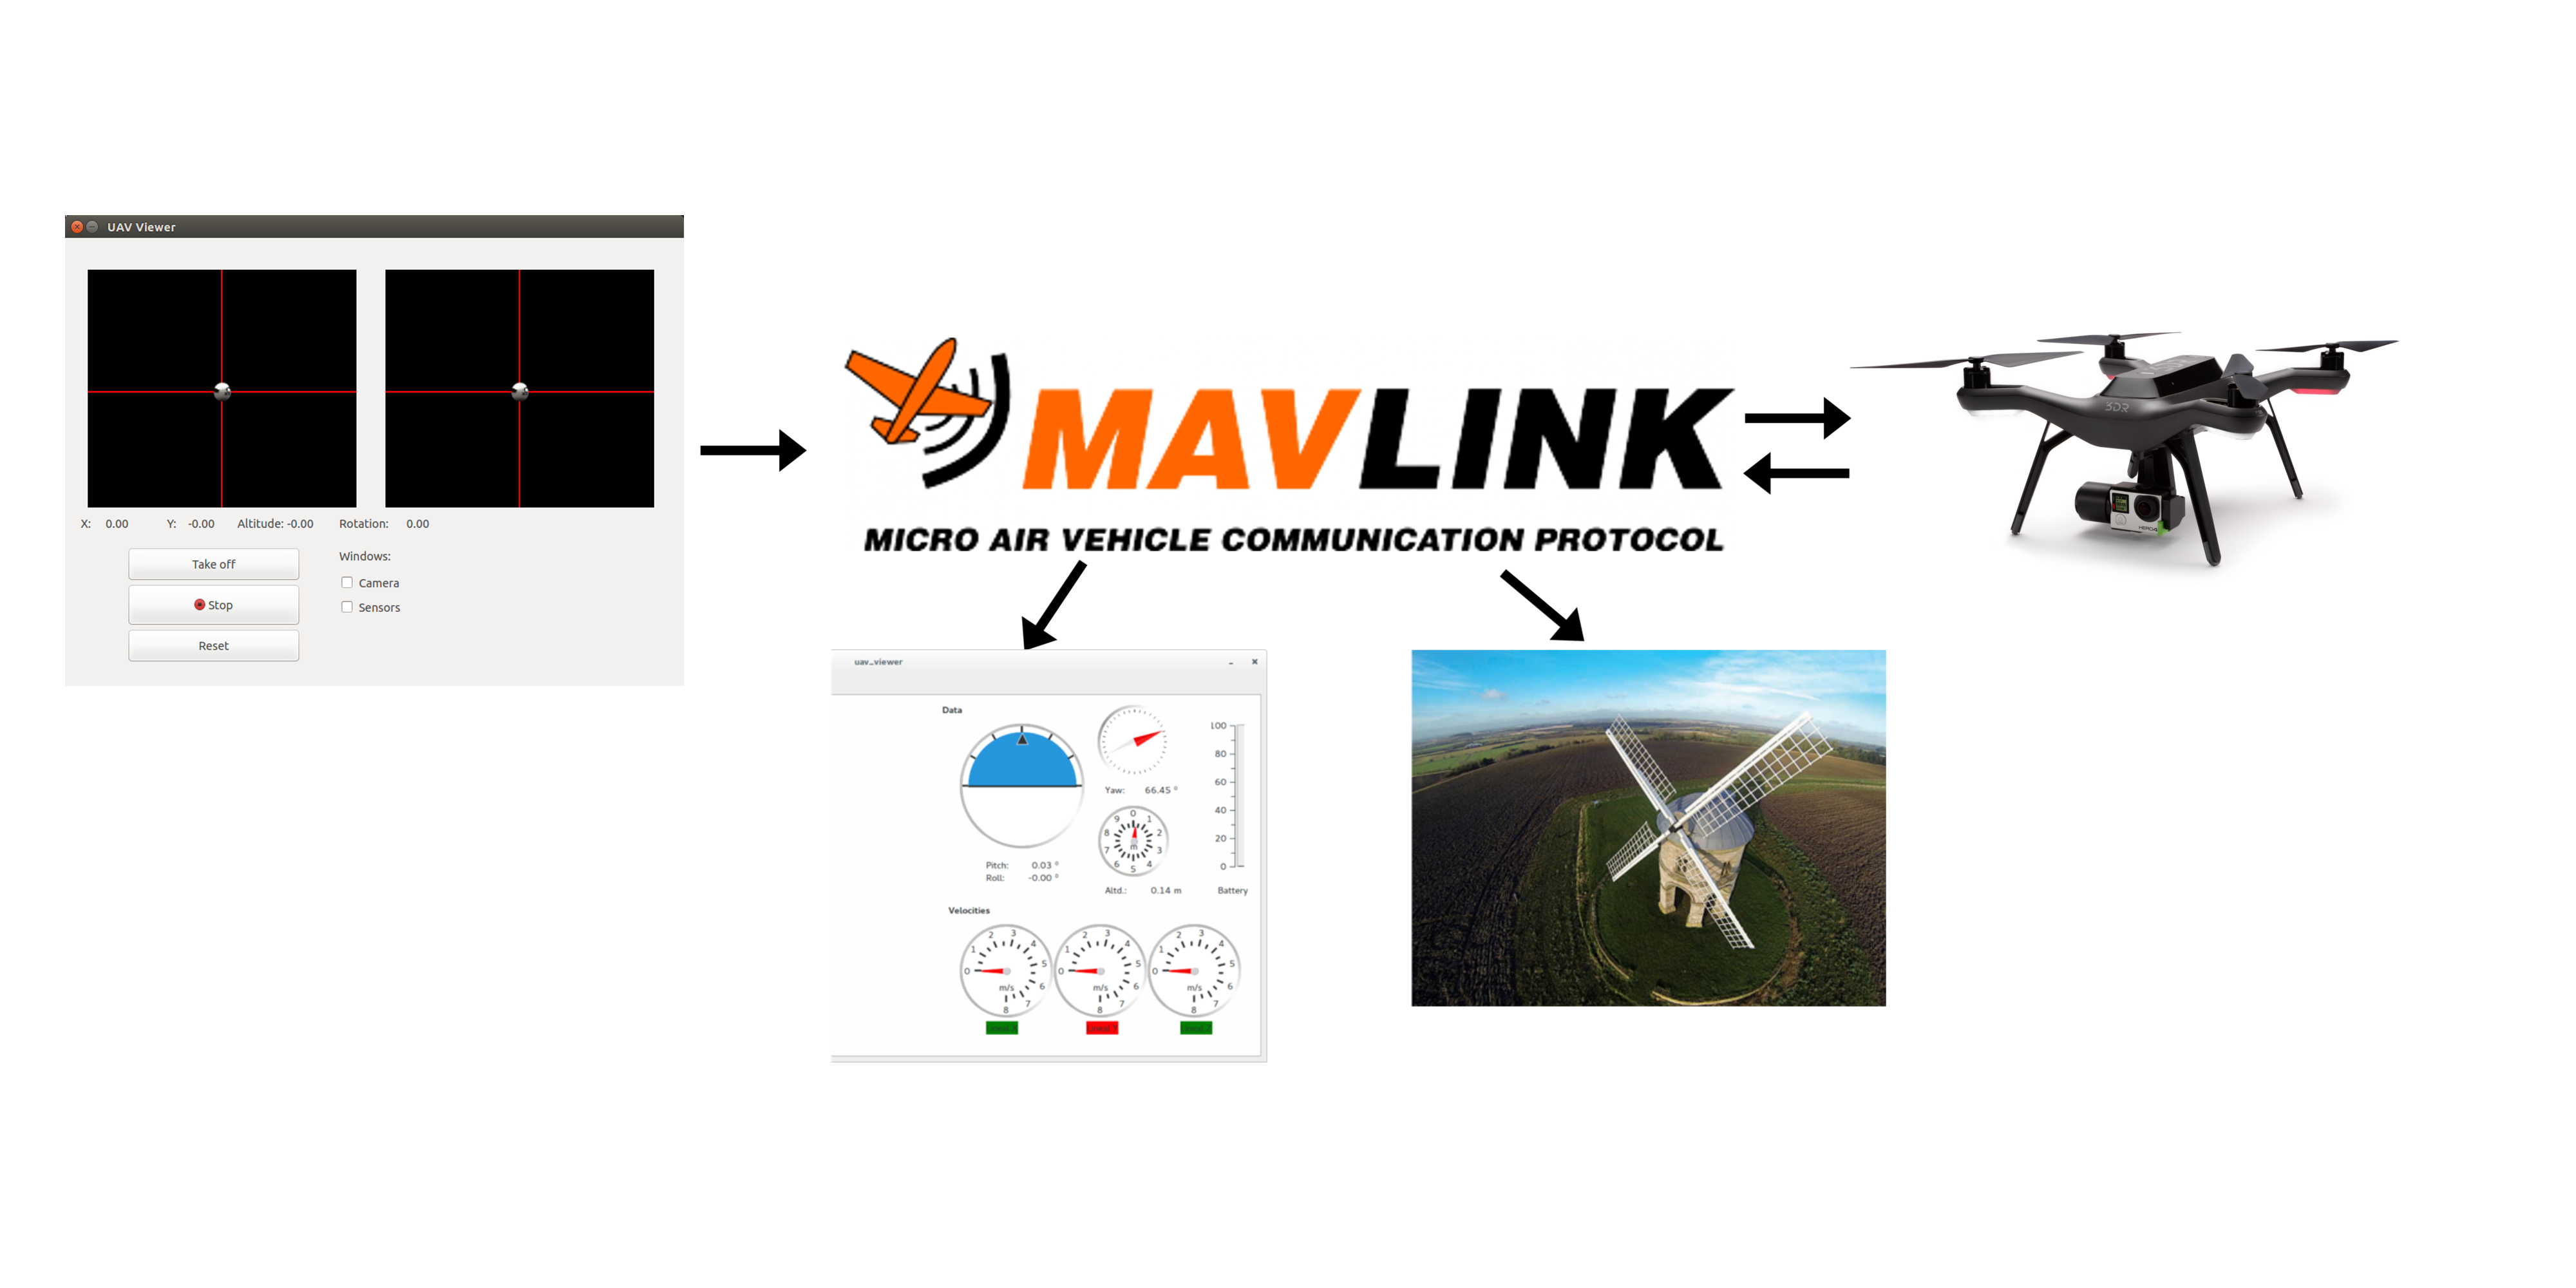
\includegraphics[scale=0.1]{imagenes/diagramaComunicacionServerDron1.png}
  \caption{Diagrama comunicación}
  \label{fig:diagramaComunicacionServerDron1}
\end{figure}


A continuación vamos a dividir en distintas fases el contenido de este driver y su ejecución:

\begin{itemize}
\item Diseño
\item Pre-Configuración
\item Implementación
\end{itemize}

\section{Diseño}
\label{Diseno}
MAVLinkServer es un controlador basado en el software MAVProxy y desarrollado para actuar como un middleware de traducción. Ha sido diseñado como un controlador JdeRobot en lenguaje Python. Este componente también es responsable de mantener la comunicación canales abiertos y actualizados, tanto en sentido ascendente como descendente. MAVLinkServer se basa en el analizador MAVProxy, la parte del programa que está a cargo de la administración de los mensajes de MAVLink. Establece la conexión con el piloto automático Pixhawk, Mantiene el canal de comunicación operativo, adquiere, interpreta mensajes, crea y envía mensajes nuevos con la información solicitada u ordenada por la aplicación.

El código desarrollado está principalmente a cargo de la gestión de las interfaces JdeRobot. Es capaz de manejar la información proporcionada por el lado de MAVProxy. Regula la creación y modificación de las clases donde la información se almacena temporalmente y abre canales de comunicación ICE para hacer que el componente sea utilizable para aplicaciones JdeRobot.
Estos dos lados del componente proporcionan un controlador fiable y multi-compatible con las características de ICE; MAVLinkServer puede conectarse con aplicaciones escritas en otros diferentes idiomas, como C ++, Python o Java, a través de las interfaces de JdeRobot. La figura \ref{fig:mavLinkJdeRobot} representa un esquema de los bloques dentro de MAVLinkServer y sus conexiones a otros componentes.

\begin{figure}[H]
  \centering
  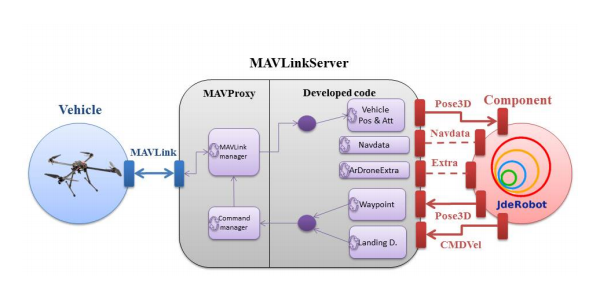
\includegraphics[scale=0.65]{imagenes/DiagramaMavLinkJdeRobot.png}
  \caption{Diagrama bloques MavLink-JdeRobot}
  \label{fig:mavLinkJdeRobot}
\end{figure}

MAVProxy es un sistema de comunicación grupal totalmente funcional  para drones. Es un sistema minimalista, portátil y extensible para cualquier UAV que soporte el protocolo MAVLink. Tiene una serie de características clave, que incluyen la capacidad de reenviar mensajes de UAV a través de la red a través de UDP o TCP a otros programas de estación terrestre en otros dispositivos.

\begin{itemize}
\item Es una aplicación de línea de comandos y consola. Hay complementos incluidos en MAVProxy para proporcionar una GUI básica.
\item Está escrito en Python.
\item Es de código abierto.
\item Es portátil; debería ejecutarse en cualquier sistema operativo POSIX con python, pyserial y función llamadas, lo que significa Linux, OS X, Windows y otros.
\item Admite módulos cargables, y tiene módulos para admitir consolas, mapas en movimiento, joysticks, seguidores de antena, etc.
\end{itemize}

MavProxy es un componente multithread (maneja varios hilos de ejecución simultáneamente). El flujo de la información y la operación del controlador seguir la siguiente ruta de la tarea:

\begin{itemize}
\item El controlador comienza a ejecutar todos los hilos diferentes, abriendo su comunicación canales y definiendo la información que estaría en cada uno. Hace uso de dos canales de comunicación basados en Pose3D, uno para publicar la posición del vehículo y actitud y otra para recibir órdenes de puntos de referencia; y un CMDVel canal para los comandos de aterrizaje.
\item Los mensajes de MAVLink entran en el controlador y se interpretan para obtener la información de posición y actitud del vehículo. Adquirida esta  información se trata para transformarla en estándares JdeRobot (Pose3D). Latitud y la longitud se transforman en coordenadas xyz globales, utilizando WGS84 como la Tierra modelo, y la actitud de ángulos de Euler se transforman en cuaterniones.
\item Pose3D está escrito en las clases locales correspondientes de forma controlada, haciendo uso de lock (librería que nos permite excluir ciertas variables para su uso).
\item Las clases se publican en los canales de ICE correspondientes a medida que se ejecutan los hilos, para permitir que otros componentes de JdeRobot puedan acceder a ellos.
\item Los comandos de aterrizaje se reciben a través de Extra y comandos de velocidad a través de CmdVel. La información se extrae de las clases correspondientes.
\item Los comandos se traducen a mensajes MAVLink y se envían a la placa Pixhawk.
\end{itemize}

Se puede ver que cada subproceso tiene una tarea pero no tienen la misma carga de trabajo.
Por esta razón, el tiempo del ciclo de control de cada hilo es diferente. A pesar de la los hilos tienen diferentes ritmos, el componente funciona con éxito en todas sus diferentes tareas.

MAVLink admite tipos de datos enteros de tamaño fijo, números de punto flotante de precisión simple IEEE 754, matrices de estos tipos de datos (por ejemplo, char [10]) y el campo especial de conversión de MavLink, que se agrega automáticamente mediante el protocolo. Estos tipos están disponibles:

\begin{multicols}{3}
\begin{itemize}
\item char
\item uint8
\item int8
\item uint16
\item int16
\item uint32
\item int32
\item uint64
\item int64
\end{itemize}
\end{multicols}

Estos paquetes que se envían tienen la estructura de la imagen \ref{fig:protocoloMavlink}, y en la tabla \ref{tablaMavLinkProtocolo} se hace referencia a cada uno de los campos con una breve explicación de cada uno de ellos:

\clearpage
\begin{figure}[H]
  \centering
  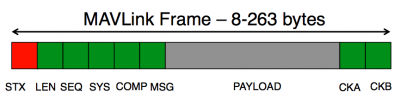
\includegraphics[scale=0.65]{imagenes/protocoloMavLink.png}
  \caption{Protocolo Mavlink}
  \label{fig:protocoloMavlink}
\end{figure}

\begin{center}
	\label{tablaMavLinkProtocolo}
    \begin{tabular}{ | p{2cm} | p{2cm} | p{3cm} | p{5cm} |}
    \hline
    Índice del byte & Contenido & Valor & Explicación \\ \hline
    0 & Señal inicio paquete & 0xFE  & Indica el inicio de un nuevo paquete. \\ \hline
     1 & Longitud de la carga	& 0 - 255 & Indica la longitud de los datos que lleva. \\ \hline
     2 & Secuencia del paquete & 0 - 255 & Cada componente cuenta con su propia secuencia. Permite detectar paquetes perdidos. \\
    \hline
    3 & ID del sistema & 1 - 255 & ID del sistema emisor. Permite diferenciar MAVs en la misma red. \\
    \hline
    4 & ID del componente & 0 - 255	& ID del componente emisor. Permite diferenciar componentes en el mismo sistema, por ejemplo la IMU y la cámara.\\
    \hline
    5 & ID del mensaje	& 0 - 255 & Permite identificar los datos del paquete para su correcta decodificación.\\
    \hline
     6 to (n+6)  & Datos	& (0 - 255) bytes & Datos del mensaje, depende del ID del mensaje.\\
    \hline
   	(n+7) to (n+8) & Checksum &  & El checksum  incluye MAVLINK-CRC-EXTRA (protege el paquete de una decodificación errónea). \\ 
    \hline
    \end{tabular}
\end{center}
\clearpage

%% \section{Módulos MavLink}
%% \begin{enumerate}
%% \label{comandos}
%% \item reboot: Reinicia el dron.
%% \item arm: Habilita los medidores propios del dron. Ejemplo de ejecución: [check %% all|baro|compass|gps|ins|params|rc|voltage|battery],uncheck %% [all|baro|compass|gps|ins|params|rc|voltage|battery],list,throttle,safetyon,safetyoff] (arm throttle arranca hélices del dron)
%% \item disarm: Detiene los motores del dron.
%% \item takeoff: Despegue del dron.
%% \item land: Aterrizaje del dron.
%% \item mode: Cambia el modo de vuelo.
%% \item velocity: Establece una velocidad en los ejes x,y,z. Ejemplo de ejecución: velocity 1 0 0
%% \item parachute: Habilita un aterrizaje del dron si pierde conexión o la batería es baja. Ejemplo de ejecución: parachute [enable|disable|release]
%% \item bat: Muestra batería del dron.
%% \item alt: Muestra altitud del dron.
%% \end{enumerate}

\section{Pre-Configuración}
\label{Pre-Configuracion}
En este apartado nos vamos a centrar en explicar todo lo relacionado con los pasos a seguir para realizar una configuración, que nos puede ofrecer dependiendo de este tipo de configuración y todas las librerías que tenemos a nuestra disposición.

Para llevar a cabo esta configuración del servidor debemos tener en cuenta la existencia de una serie de ficheros, llamados módulos (en lenguajes como java, suelen conocerse con el nombre de librerías), que cada uno de ellos nos va a facilitar una utilidad diferente, que pueden ir desde conocer la batería, altura del dron o configurar una web-cam.

Estos módulos se pueden descargar desde el repositorio oficial de MavLink o crear una librería propia e implementarla. En el siguiente código que se muestra se puede ver como esta implementa obtener la información de la batería a través del voltaje que desprende:
\footnote{\url{https://github.com/ArduPilot/MAVProxy}}.

{\scriptsize
\begin{verbatim}
    def vcell_to_battery_percent(self, vcell):
        '''convert a cell voltage to an approximate
        percentage battery level for a LiPO'''
        if vcell > 4.1:
            # above 4.1 is 100% battery
            return 100.0
        elif vcell > 3.81:
            # 3.81 is 17% remaining, from flight logs
            return 17.0 + 83.0 * (vcell - 3.81) / (4.1 - 3.81)
        elif vcell > 3.2:
            # below 3.2 it degrades fast. It's dead at 3.2
            return 0.0 + 17.0 * (vcell - 3.20) / (3.81 - 3.20)
        # it's dead or disconnected
        return 0.0
\end{verbatim}}

El fichero de configuración que usa el servidor únicamente se limita a establecer los puertos mediante los cuales se va a realizar la comunicación de cara a un usuario. Esta comunicación la realiza mediante las interfaces ICE que permite la comunicación con el servidor, pudiendo así recibir datos de sensores y motores, y enviar las instrucciones de velocidad necesarias en cada momento.

\section{Implementación}
\subsection{Script de arranque}
\label{Script de arranque}

El script de arranque se encargara de ejecutar todos los comandos previos y el servidor. El script se encuentra en MAVProxy/MAVProxyWinLAN.sh, deberemos averiguar la IP que levanta el dron, en nuestro caso, con el 3DR Solo, dicha IP la levanta el mando como hemos comentado en la introducción de este capitulo. Deberemos modificar el script con la IP del dron a la que nos hayamos conectado y ejecutarlo sin parámetros adicionales. El fichero README del repositorio contiene una descripción mas detallada de un ejemplo de ejecución.

Se necesita tener preinstalado tanto pyserial como una versión de pyvmavlink superior a la 1.1.50. Se realiza una descarga de todos los módulos, construye un directorio llamado MavProxy.egg en /home/USER/.local/python3.5/site-packages con el fin de tener almacenados todos los paquetes necesarios y con permisos suficientes. 

A través de estos paquetes generados es posible acceder a los comandos que nos proporciona MavLink. A continuación se proporciona un listado de los posibles comandos opcionales que se pueden añadir al script de arranque y una breve explicación de cada uno de ellos (todos los comandos deben introducirse a continuación con "--" por delante):

\begin{multicols}{2}
\begin{itemize}
\item master: Puerto maestro MAVLink y baudrate opcional. Por defecto=[].
\item udp: Arranca el servidor udp. Por defecto se elige TCP.
\item tcp: Arranca el servidor tcp. Por defecto se elige TCP.
\item out: Puerto de salida MAVLink. Por defecto=[].
\item baudrate: Por defecto=57600.
\item sitl(Software in the loop): Puerto de salida, esta opción únicamente es necesaria en caso de no tener disponible un dron.
\item streamratedest: MAVLink stream rate. Por defecto=4.
\item source-system: Código fuente MAVLink. Por defecto=255.
\item source-component: Componente origen MAVLink. Por defecto=0.
\item target-system: Sistema destino MAVLink. Por defecto=0.
\item target-component: Componente destino MAVLink. Por defecto=0.
\item logfile: Fichero de logs. Por defect=mav.tlog
\item append-log (También aceptado "-a"): Añadir al fichero de log ya existente. Por defecto=False.
\item continue (También aceptado con "-c"): Continua el log. Por defecto=False.
\item quadcopter: Usar acciones de control para cuadricopteros. Por defecto=False.
\item setup: Arrancar en modo setup. Por defecto=False.
\item nodtr: Deshabilitar DTR(Data Terminal Ready). Por defecto=False.
\item show-errors: Mostrar errores MAVLink. Por defecto=False.
\item speech: Usar texto para hablar. Por defecto=False.
\item aircraft: Establecer nombre para el dron (Visual en mensajes). Por defecto=None.
\item cmd: Comandos a ejecutar tras el arranque. Por defecto=None.
\item console: Usar consola GUI para introducir comandos. 
\item map: Carga un mapa de la zona.
\item load-module: Carga un modulo especifico, puede ser utilizado tantas veces como sea necesario separando con ","). Por defecto=[].
\item mav09: Usa protocolo MavLink 0.9. Por defecto=False.
\item auto-protocol: Auto detecta versión de protocolo MAVLink. Por defecto=False.
\item nowait: No realiza comunicación continua con el dron (HearthBeat). Por defecto=False.
\item dialect: Dialecto MavLink. Por defecto=ardupilotmega.
\item rtscts: Habilita control de comunicación vía RTS/CTS.
\item moddebug  type=int, help="module debug level default=0
\item mission: Nombre de la misión. Por defecto=None.
\item daemon: Arranca en modo daemon, no muestra shell interactiva.
\item profile: Arranca el Yappi python profiler.
\item state-basedir: Directorio base para logs. Por defecto=None.
\item version: Muestra información sobre la versión.
\item default-modules: Módulos por defecto al iniciar. Por defecto=log, wp, rally, fence, param, relay, tuneopt, arm, mode, calibration, rc, auxopt, misc, cmdlong, battery, terrain, output.
\end{itemize}
\end{multicols}

\subsection{MavLinkServer}
En el arranque del servidor se cargan los paquetes de antes comentados y a partir de los cuales se podrán proporcionar funcionalidades, un ejemplo es el modo consola, el cual nos permite controlar al dron a partir de comandos definidos en la siguiente lista:


\begin{itemize}
\label{comandos}
\item reboot: Reinicia el dron.
\item arm: Habilita los medidores propios del dron. Ejemplo de ejecución: check (all|baro|compass|gps|ins|params|rc|voltage|battery),uncheck (all|baro|compass|gps|ins|params|rc|voltage|battery),list,throttle,safetyon,safetyoff (arm throttle arranca hélices del dron)
\item disarm: Detiene los motores del dron.
\item takeoff: Despegue del dron.
\item land: Aterrizaje del dron.
\item mode: Cambia el modo de vuelo.
\item velocity: Establece una velocidad en los ejes x,y,z. Ejemplo de ejecución: velocity 1 0 0
\item parachute: Habilita un aterrizaje del dron si pierde conexión o la batería es baja. Ejemplo de ejecución: parachute [enable|disable|release]
\item bat: Muestra batería del dron.
\item alt: Muestra altitud del dron.
\end{itemize}

Para llevar a cabo esta carga el primer paquete que se carga es "Link", este paquete se encarga de la conexión entre el servidor y el dron. Es necesario conocer la dirección IP que levanta este dron, que ya habremos configurado en el paso \ref{Script de arranque}. Tras lograr la conexión se establece un periodo de "checkeo" necesario para no perder la conexión con el dron en caso de llegar a una distancia límite o un fallo de conexión, en cuyo caso se procede a detenerse el dron. Esto se debe a periódicamente se debe realizar una comunicación entre el dron y el servidor, aunque no se llegue a mandar ningún comando, ya sea de velocidad o algún tipo de acción, el servidor por su parte comunicara que aun esta conectado. Después de un tiempo sin conexión, aproximadamente unos 10-15 segundos, el dron procederá a realizar un despegue. 

{\scriptsize
\begin{verbatim}
def periodic_tasks():
    '''run periodic checks'''
    if mpstate.status.setup_mode:
        return

    if (mpstate.settings.compdebug & 2) != 0:
        return

    if mpstate.settings.heartbeat != 0:
        heartbeat_period.frequency = mpstate.settings.heartbeat

    if heartbeat_period.trigger() and mpstate.settings.heartbeat != 0:
        mpstate.status.counters['MasterOut'] += 1
        for master in mpstate.mav_master:
            send_heartbeat(master)

    if heartbeat_check_period.trigger():
        check_link_status()

    set_stream_rates()

    # call optional module idle tasks. These are called at several hundred Hz
    for (m,pm) in mpstate.modules:
        if hasattr(m, 'idle_task'):
            try:
                m.idle_task()
            except Exception as msg:
                if mpstate.settings.moddebug == 1:
                    print(msg)
                elif mpstate.settings.moddebug > 1:
                    exc_type, exc_value, exc_traceback = sys.exc_info()
                    traceback.print_exception(exc_type, exc_value, exc_traceback,
                                              limit=2, file=sys.stdout)

        # also see if the module should be unloaded:
        if m.needs_unloading:
            unload_module(m.name)
\end{verbatim}}
            
Al acabar toda la carga de los módulos establecemos la conexión con los puertos necesarios con JdeRobot para poder pilotar el dron. Los componentes que usamos son Pose3D, CMDVel y Extra. Para cada uno de ellos vamos a necesitar crear 2 threads, uno para establecer la conexión con un sistema externo, en nuestro caso será el visor UavViewer, y otro para recibir los comandos que nos deseen enviar por el canal. Cada componente lo necesitaremos por los siguientes motivos:

{\scriptsize
\begin{verbatim}

def load_module(modname, quiet=False):
    '''load a module'''
    modpaths = ['MAVProxy.modules.mavproxy_%s' % modname, modname]
    for (m,pm) in mpstate.modules:
        if m.name == modname:
            if not quiet:
                print("module %s already loaded" % modname)
            return False
    for modpath in modpaths:
        try:
            m = import_package(modpath)
            imp.reload(m)
            module = m.init(mpstate)
            if isinstance(module, mp_module.MPModule):
                mpstate.modules.append((module, m))
                if not quiet:
                    print("Loaded module %s" % (modname,))
                return True
            else:
                ex = "%s.init did not return a MPModule instance" % modname
                break
        except ImportError as msg:
            ex = msg
            if mpstate.settings.moddebug > 1:
                import traceback
                print(traceback.format_exc())
    print("Failed to load module: %s. Use 'set moddebug 3' in the MAVProxy console to enable traceback" % ex)
    return False
\end{verbatim}}

\begin{itemize}
\item CMDVel: Este componente nos dará lo necesario para poder mover el dron en los ejes x,y,z y sobre el yaw. La velocidad máxima que se le puede dar al dron a través del interfaz UavViewer en cada dirección viene dado en una escala de 0 a 1.  
\item Extra: Este componente nos dará la facilidad de despegar y de aterrizar. Debido al protocolo MavLink, el sistema de despegue se compone en 3 fases, que con nuestro UavViewer se agrupan todas ellas. Durante la fase de despegue el dron no admite ningún comando a excepción del comando "land" para aterrizar, o en caso del despegue, para detener el despegue.  Este despegue dura aproximadamente unos 10 segundos hasta que se estabiliza en el aire por motivos de seguridad. \begin{enumerate}
						\item El arranque de las hélices. 
                        \item Despegue del dron.
                        \item Habilitar comandos de velocidad.
						\end{enumerate}
\item Pose3d: Este componente nos indicara la posición del dron en todo momento, así como su orientación y altitud. Esta conexión nos va a servir tanto a la hora de aterrizar y despegar usando el otro componente comentado Extra, para saber si puede aterrizar en un determinado momento, o debe disminuir su altura antes de parar los motores, como también a la hora de usar el otro componente CMDVel, ya que si necesitamos girar el dron sobre el yaw, MavLink tiene el inconveniente de necesitar ordenes de velocidad con grados absolutos de -180 a 180º, de modo que es necesario saber la posición en cada momento del dron para indicarle un movimiento relativo. La conversión se realiza de la siguiente forma:

{\scriptsize
\begin{verbatim}
angular = Pose3D2send.q3 + CMDVel.angularZ
if angular > 1:
	angular = angular - 2
elif angular < -1:
	angular = angular + 2
angularZstring = str(angular*180)
\end{verbatim}}

A través de la posición absoluta actual y con la orden que nos indican mediante el componente CMDVel, calcularemos el punto destino al cual debe rotar el dron. 

\end{itemize}

\clearpage
MAVLinkServer lanza varios hilos para canales de comunicación ICE, uno para cada tipo de información. A pesar de que solo Pose3D, CMDVel y Extra deben ser realmente utilizados, el driver ofrece las interfaces restantes para compatibilidad y usos futuros.

\begin{figure}[H]
  \centering
  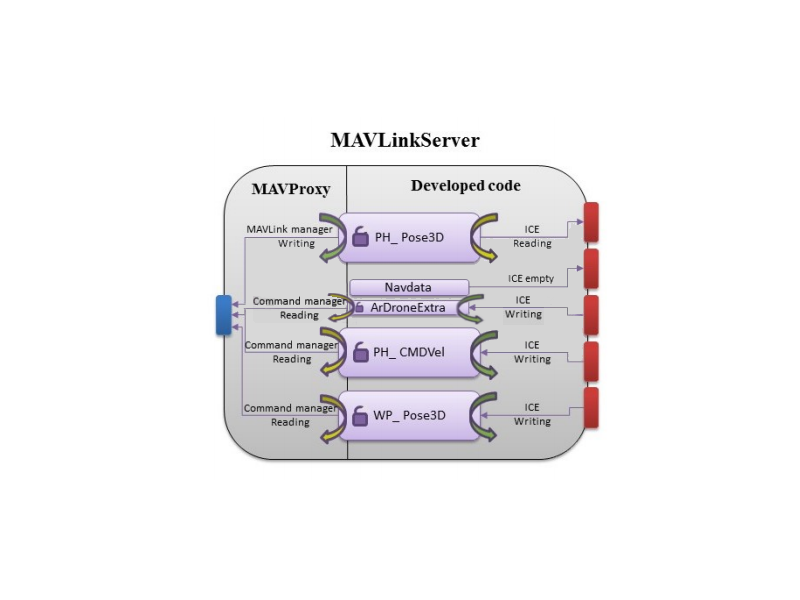
\includegraphics[scale=0.7]{imagenes/MavProxyPorDentro.png}
  \caption{MavProxy gestión}
  \label{fig:MavProxyInside}
\end{figure}

Cada subproceso hace uso de su propia función donde se realiza la configuración de ICE.
Allí se realiza la publicación de ICE y es importante garantizar qué datos se envían, para que otras aplicaciones obtengan la información correctamente y garanticen la compatibilidad.
El mismo procedimiento se realiza para todas las interfaces.

{\scriptsize
\begin{verbatim}
	mpstate.status.thread = threading.Thread(target=main_loop, name='main_loop')
    mpstate.status.thread.daemon = True
    mpstate.status.thread.start()

    #Open an ICE TX communication and leave it open in a parallel threat

    PoseTheading = threading.Thread(target=openPose3DChannel, args=(PH_Pose3D,), name='Pose_Theading')
    PoseTheading.daemon = True
    PoseTheading.start()

    # Open an ICE RX communication and leave it open in a parallel threat

    CMDVelTheading = threading.Thread(target=openCMDVelChannel, args=(PH_CMDVel,), name='CMDVel_Theading')
    CMDVelTheading.daemon = True
    CMDVelTheading.start()

    # Open an ICE TX communication and leave it open in a parallel threat

    CMDVelTheading = threading.Thread(target=openExtraChannel, args=(PH_Extra,), name='Extra_Theading')
    CMDVelTheading.daemon = True
    CMDVelTheading.start()

    # Open an ICE channel empty

    CMDVelTheading = threading.Thread(target=openNavdataChannel, args=(), name='Navdata_Theading')
    CMDVelTheading.daemon = True
    CMDVelTheading.start()

    # # Open an MAVLink TX communication and leave it open in a parallel threat
    #
    PoseTheading = threading.Thread(target=sendCMDVel2Vehicle, args=(PH_CMDVel,PH_Pose3D,), name='TxCMDVel_Theading')
    PoseTheading.daemon = True
    PoseTheading.start()


    # Open an ICE TX communication and leave it open in a parallel threat

    PoseTheading = threading.Thread(target=openPose3DChannelWP, args=(WP_Pose3D,), name='WayPoint_Theading')
    PoseTheading.daemon = True
    PoseTheading.start()

    # Open an MAVLink TX communication and leave it open in a parallel threat

    PoseTheading = threading.Thread(target=sendWayPoint2Vehicle, args=(WP_Pose3D,), name='WayPoint2Vehicle_Theading')
    PoseTheading.daemon = True
    PoseTheading.start()

    # Open an MAVLink TX communication and leave it open in a parallel threat

    PoseTheading = threading.Thread(target=landDecision, args=(PH_Extra,), name='LandDecision2Vehicle_Theading')
    PoseTheading.daemon = True
    PoseTheading.start()
   
\end{verbatim}}

MAVproxy está constantemente manejando los mensajes MAVLink en un hilo paralelo en un bucle infinito. Este componente lo aprovecha y refresca la información del sensor necesario. Como un controlador de alto nivel, este programa no interfiere con la fusión de datos realizado por Pixhawk y confía en su rendimiento, cuya fiabilidad ha sido ampliamente probado.
